\documentclass[12pt]{article}
\usepackage{polski}
\usepackage{lmodern}
\usepackage[utf8]{inputenc}
\usepackage{tabto}
\usepackage{indentfirst} %pierwszy akapit posiada wcięcie
\usepackage{graphicx}
\title{Równania nieliniowe - projekt}
\author{Natalia Wojtania i Grzegorz Chojnacki}
%\date{}
\begin{document}
\maketitle

\section{Zadanie}
\subsection{Tytuł}
Tytuł zadania to ,,Przybliżone rozwiązywanie równań nieliniowych".
\subsection{Treść}
Napisz program, który rozwiązuje równanie: $$4x^{3} + 5x^{2} + 6x - 7 = 0$$\emph{metodą siecznych.}
\subsection{Metoda}
W programie należy wykorzystać metodę siecznych.
\subsubsection{Opis metody}

Metoda siecznych (interpolacji liniowej) polega na przyjęciu, że funkcja ciągła na dostatecznie małym odcinku w przybliżeniu zmienia się w sposób liniowy. Można wtedy na odcinku $[a,b]$ krzywą $y=f(x)$ zastąpić sieczną. Za przybliżoną wartość pierwiastka przyjmuje się punkt przecięcia siecznej z osią odciętych $OX$. Miejsce przecięcia tej prostej z osią $X$ jest przybliżonym wynikiem szukanego miejsca zerowego, o ile różnica bezwzględna wartości z dwóch ostatnich iteracji jest mniejsza od założonej dokładności.  Metoda ta wymaga ustalenia na przedziale $[a,b]$ dwóch punktów startowych $x_0$ i $x_1$.\\
Metodę siecznych dla funkcji $f(x)$, mającej pierwiastek w przedziale $[ a , b ]$ można zapisać następującym wzorem rekurencyjnym:

 $$x_{k+1}=x_k - \frac{f(x_k)(x_k-x_{k-1})}{f(x_k)-f(x_{k-1})}, k \geq 1$$ i $$x_0=a, x_1=b, $$ gdzie w każdym kroku $ x_{k+1}$ to miejsce zerowe siecznej wykresu $y=f(x)$ w punktach $(x_{k-1},f(x_{k-1}))$ oraz$ (x_{k},f(x_{k})) $, czyli prostej $$y=\frac{f(x_k)-f(x_{k-1})}{x_k-x_{k-1}}(x-x_k)+f(x_k)$$
\subsubsection{Przykład}
Dla równania $x^3-2x-5=0$ rozważanego na przedziale $[a,b]=[2,3]$ przybliżyć rozwiązanie wartością $x_k$ wyznaczoną metodą siecznych z\\
$x_0=a, x_1=b$ oraz dokładnością $\epsilon = 0.5.$
\\ \\
$ x_2=x_1 - \frac{f(x_1)(x_1-x_{0})}{f(x_1)-f(x_{0})}$
\\ \\
 Mamy $ x_{0}=2,$ i $x_{1}=3, f(x_1)=f(3)=16, f(x_0)=f(2)=-1$
\\$x_2=3-\frac{16(3-2)}{16-(-1)}=2 \frac{1}{17}, |x_2 - x_1|\approx 0,94 > \epsilon,$
$f(x_2)=f(2 \frac{1}{17})\approx-0.39$ $x_3=2 \frac{1}{17}-\frac{-0.39(-0,94)}{-0.39-16}\approx2.08, |x_3 - x_2|\approx 0.02<\epsilon$
\\Zatem przybliżone rozwiązanie $x_k=2.08$ oraz $k=3$
\section{Opis implementacji algorytmu}
Implementacja realizująca metodę siecznych.
\subsection{Dane wejściowe}
Na wejściu program pobiera od użytkownika wartość wyrażającą dokładność rozwiązania(epsilon) $\epsilon \in(0,1).$



\subsection{Przebieg działania}
Program wyświetla komunikat: ,,Wprowadź dokładność rozwiązania $\epsilon \in(0,1)$ ". Jeśli została wprowadzona prawidłowa wartość dokładności, to program poprzez funkcję \emph{calculate} wylicza przybliżone rozwiązanie i dzięki funkcji \emph{refresh} wyświetla je wraz z liczbą kroków.
Próba wprowadzenia nieprawidłowych danych, które weryfikowane są w programie w funkcji \emph{refresh} skutkuje wyświetleniem stosownego ostrzeżenia.
\par Następnie funkcja \emph{calculate} klasy \emph{SecantMethod} zajmuje się wyliczeniem przybliżonego rozwiązania w oparciu o podaną dokładność i przedział wyszukany za pomocą funkcji \emph{findInterval}. Szukanie przedziału zaczyna się od $[0, 1]$ i jeżeli funkcja nie przechodzi w nim przez oś $OX$, to przedział jest poszerzany.\\
Funkcja \emph{getNext}, której argumentami są $a$ i $b$ odpowiednio oznaczające $x_{k-1}$ oraz $x_{k}$ zwraca wartość poszczególnego $x_{k+1}$.
\\
Funkcja \emph{isGoodEnough} sprawdza czy różnica  $|x_k - x_{k-1}|$ jest mniejsza od podanej przez użytkownika dokładności. Jeśli tak, to kończymy przekazując wynik oraz ilość kroków. W przeciwnym wypadku liczone jest kolejne przybliżenie tak długo, aż warunek zostanie spełniony.


Wynikiem działania programu jest przybliżone rozwiązanie równania: $x_k$ oraz liczba wykonanych kroków: $k$.
\newpage
\subsection{Najważniejsze fragmenty programu}
secantMethod.js
\begin{verbatim}

class SecantMethod {
  f = x => 4*x**3 + 5*x**2 + 6*x - 7

  constructor(precision) {
    this.precision = precision
    this.interval = this.findInterval()
  }

  findInterval = (a = 0, b = 1) => this.f(a) * this.f(b) < 0
    ? [a, b]
    : this.findInterval(a - (b - a), b + (b - a))

  // a = x_{k-1}, b = x_{k}
  getNext = (a, b) => b - (this.f(b) * (b - a)) / (this.f(b) - this.f(a))
  isGoodEnough = (next, prev) => Math.abs(next - prev) < this.precision

  calculate() {
    const g = (a, b, steps = 2) => {
      const next = this.getNext(a, b)
      return this.isGoodEnough(next, b)
        ? ({ result: next, steps })
        : g(b, next, steps + 1)
    }
    return g(this.interval[0], this.interval[1])
  }
}

\end{verbatim}
\newpage
gui.js
\begin{verbatim}


const gui = new (class {
  input  = document.getElementById('input')
  result = document.getElementById('result')
  steps  = document.getElementById('steps')
  error  = document.getElementById('error')

  refresh() {
    const precision = this.getPrecision()
    if (0 < precision && precision < 1) {
      this.clearError()
      const answer = new SecantMethod(precision).calculate()
      this.result.innerText = answer.result
      this.steps.innerText  = answer.steps
    } else this.setError()
  }

  setError()   { this.error.innerText  = 'Wprowadzona wartość poza przedziałem (0, 1)' }
  clearError() { this.error.innerText  = '' }

  update = debounce(() => this.refresh(), 10)

  getPrecision = () => Number.parseFloat(this.input.value)

})()
\end{verbatim}
\newpage
\subsection{Widok działania programu}
\begin{figure}[h]
\centering
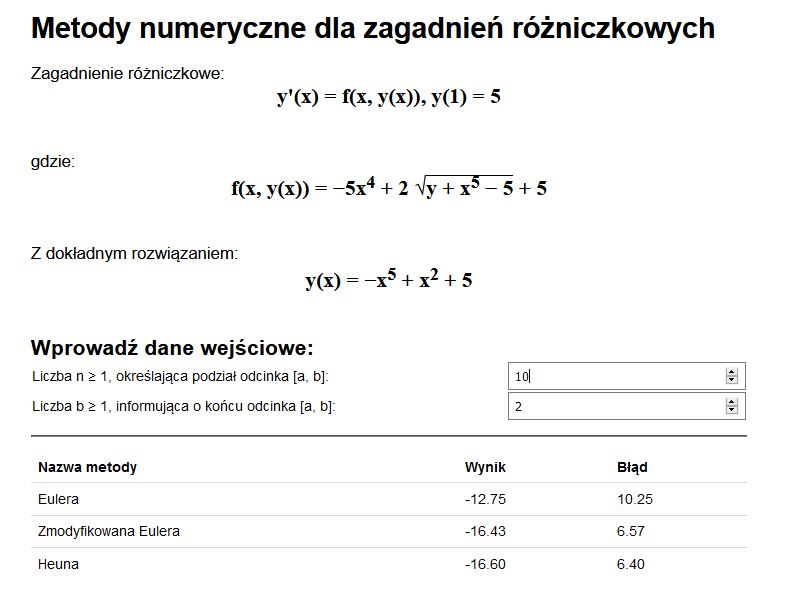
\includegraphics[scale=0.65]{correctData.jpg}
\caption{Prawidłowo wprowadzone dane}
\end{figure}

\begin{figure}
\centering
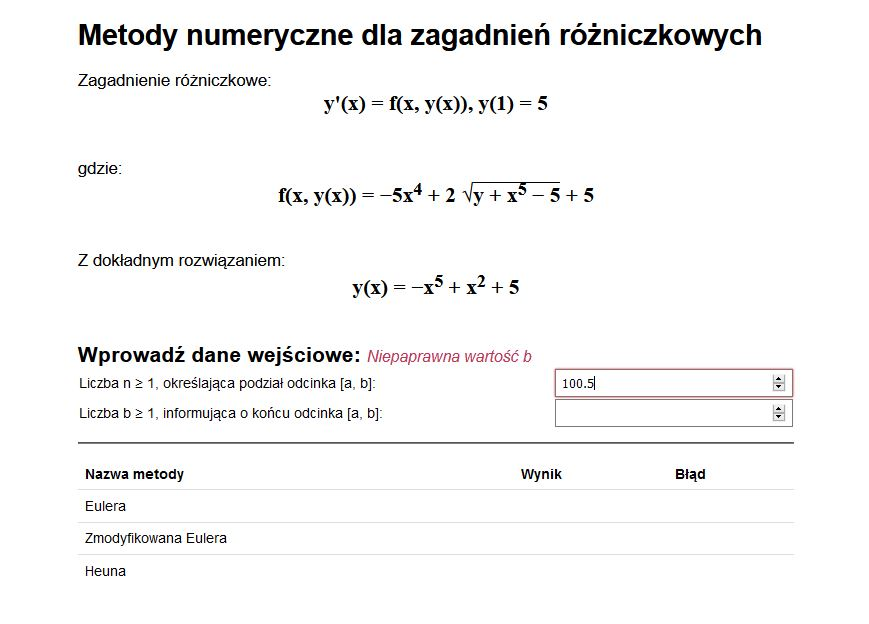
\includegraphics[scale=0.65]{wrongData.jpg}
\caption{Nieprawidłowo wprowadzone dane}
\end{figure}

\end{document}
